% ======================================================================
%  Stand-alone caption blocks for the five validation panels.
%  Include this file in the main paper or compile independently.
%  Each figure* references the panel PNG relative to the publications root.
% ======================================================================

\begin{figure*}[!htbp]
    \centering
    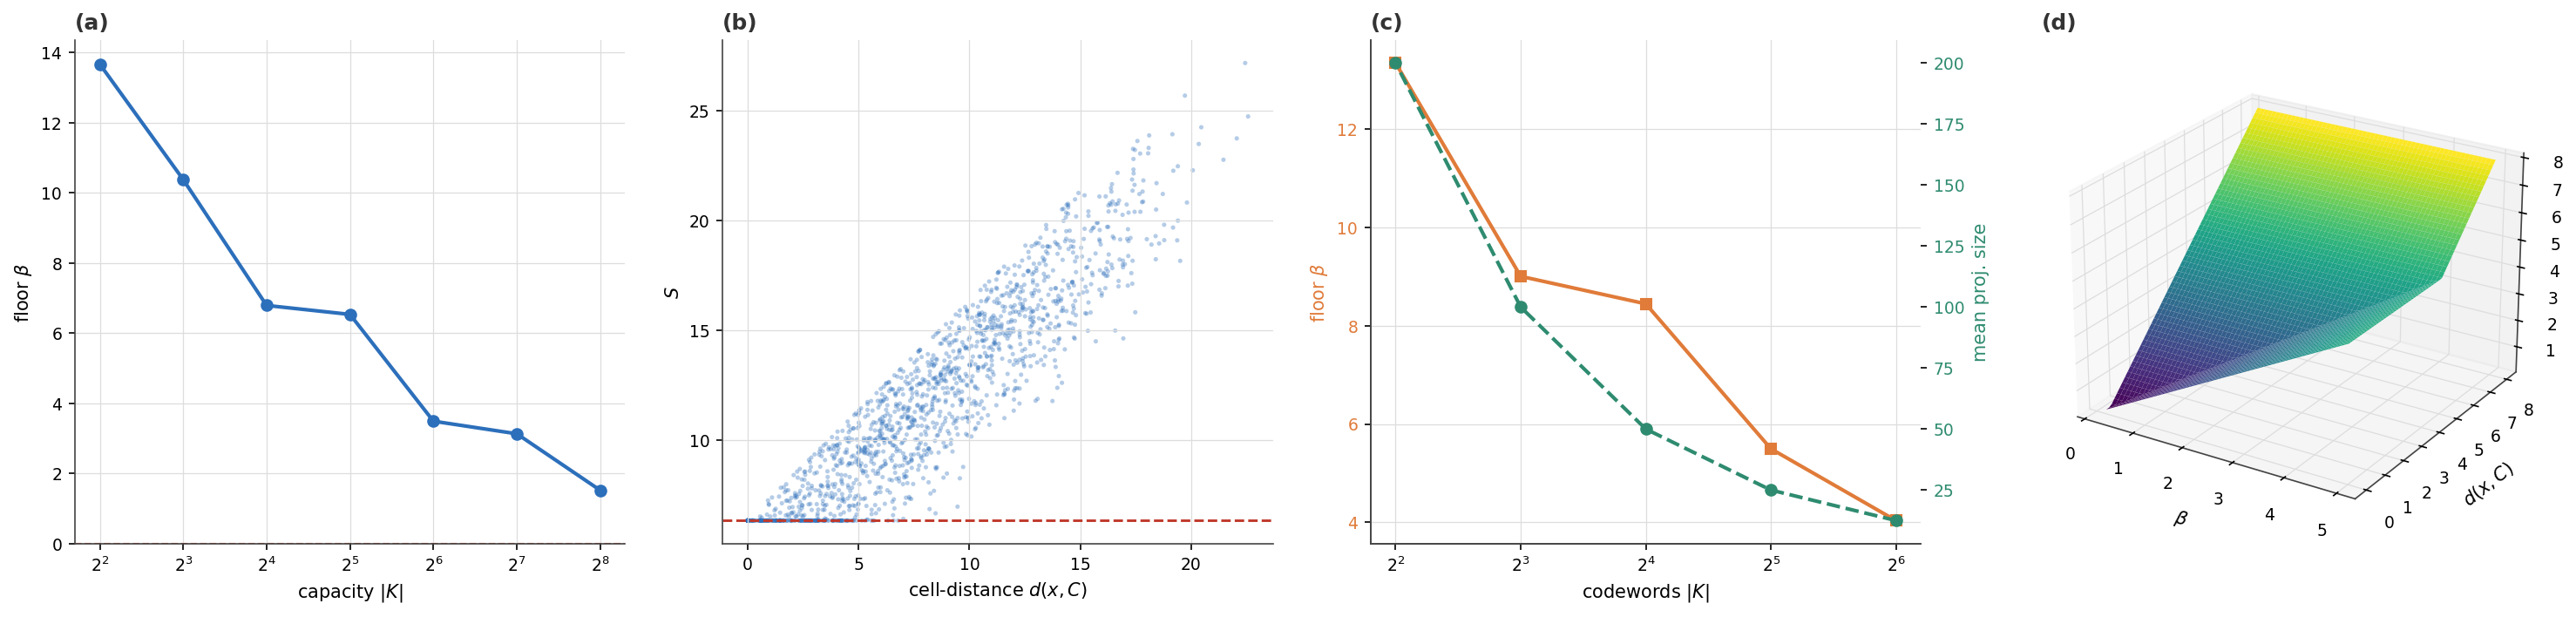
\includegraphics[width=\textwidth]{panels/panel_1.png}
    \caption{\textbf{The Floor Theorem and Granular Meaning.}
    (\textbf{A})~Floor $\beta$ on the linear $y$-axis versus codebook capacity
    $|\mathcal{K}|$ (powers of two, log $x$-axis, $2^{1}$ to $2^{7}$). The floor
    falls monotonically as capacity grows but remains strictly positive at every
    tested capacity, confirming Theorem~\ref{thm:floor} (Floor Theorem): no
    bounded receiver can attain $\beta = 0$. The curve never reaches the $x$-axis.
    (\textbf{B})~Semantic distance $S$ on the linear $y$-axis versus cell-distance
    $d(x, \mathcal{C})$ on the linear $x$-axis, across thousands of random
    (receiver, percept, cell) evaluations. Every point lies strictly above the
    floor $\beta$ (red dashed line), confirming Corollary~\ref{cor:noperfect} (No
    perfect persuasion): the functional $S(\mathcal{R}, x;\mathcal{C}) \geq \beta >
    0$ without exception.
    (\textbf{C})~Joint coarsening sweep: floor $\beta$ (orange, left $y$-axis) and
    mean projection size $|\Pi(\mathcal{D}(x))|$ (green dashed, right $y$-axis)
    versus codebook size $|\mathcal{K}|$ on the log $x$-axis ($2^{7}$ to $2^{2}$
    codewords, coarsening left to right). Both rise in lockstep as the codebook is
    coarsened, confirming Theorem~\ref{thm:nopoint} (Point-value forbidden): a
    coarser vocabulary raises the floor and enlarges the projection set together ---
    meaning grows granular, not point-like.
    (\textbf{D})~Three-dimensional $S$-surface over the $(\beta, d)$ plane: the
    surface $S(\beta, d) = \max(\beta, d) + \beta$ rises as a flat plateau above the
    floor level and then as a cone proportional to cell-distance. The flat base
    (the action-cell interior) and the rising walls (above-cell percepts) are the
    geometric content of the Floor Theorem and Cell-Truth Theorem
    (Theorem~\ref{thm:celltruth}) in one view.}
    \label{fig:panel1-floor}
\end{figure*}


\begin{figure*}[!htbp]
    \centering
    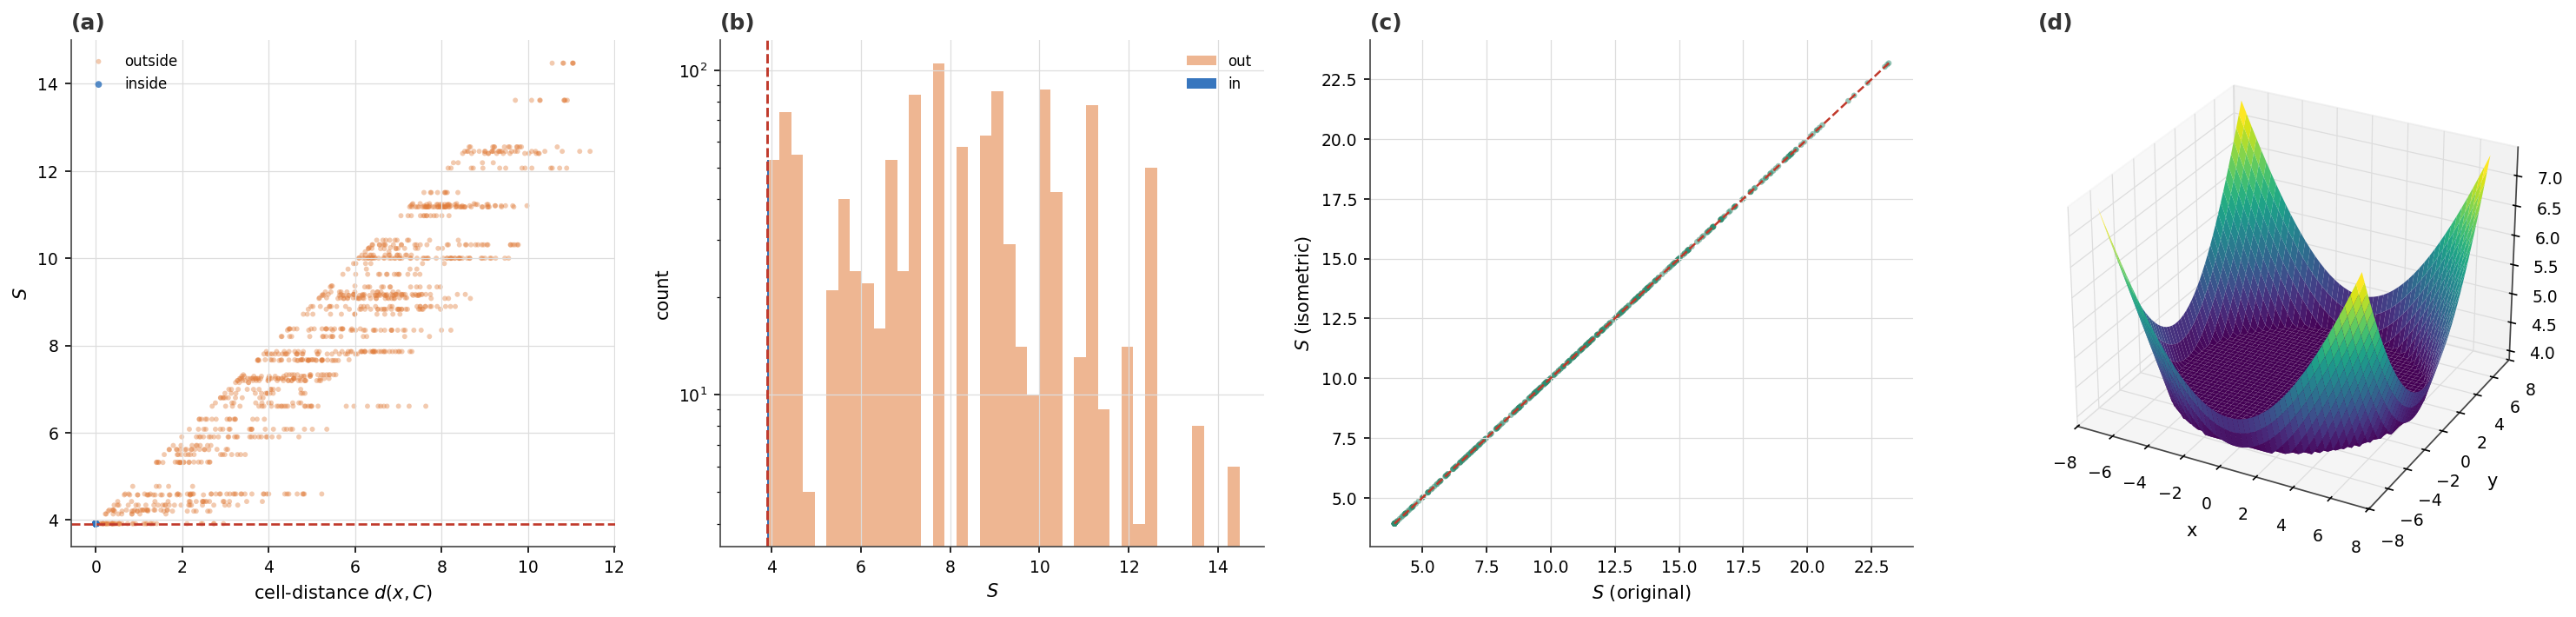
\includegraphics[width=\textwidth]{panels/panel_2.png}
    \caption{\textbf{Cell-Truth and Representational Invariance.}
    (\textbf{A})~Semantic distance $S$ on the linear $y$-axis versus cell-distance
    $d(x, \mathcal{C})$ on the linear $x$-axis, with percepts coloured by
    cell-membership (inside: filled markers; outside: open markers). In-cell
    percepts collapse to a flat band at $S = \beta$ regardless of their individual
    positions within the cell; out-of-cell percepts rise linearly above it.
    Confirms Theorem~\ref{thm:celltruth} (Cell-Truth): all percepts within an
    action-cell are receiver-indistinguishable, each attaining exactly $S = \beta$.
    (\textbf{B})~Histogram of $S$ values (log-scale $y$-axis, linear $x$-axis) for
    in-cell (dark) and out-of-cell (light) percepts over $9{,}365$ trials. The
    in-cell distribution is a spike concentrated exactly at $\beta$ with zero spread;
    the out-of-cell distribution occupies a broad range strictly above $\beta$ (red
    dashed). The log scale makes the spike visible against the taller out-of-cell
    bars. Confirms Cell-Truth and the prohibition on point-value
    (Theorem~\ref{thm:nopoint}).
    (\textbf{C})~Invariance diagonal: $S$ under isometric re-encoding ($y$-axis)
    versus original $S$ ($x$-axis) for random rotations, translations, and
    reflections across all trials. Every point lies on the identity diagonal
    (red dashed) to floating-point precision (maximum deviation
    $5.3 \times 10^{-15}$), confirming Theorem~\ref{thm:repinv}
    (Representational Invariance): cell-membership and semantic distance are
    preserved under isometric re-encoding of the carrier.
    (\textbf{D})~Three-dimensional $S$-field over the two-dimensional percept space:
    a bowl whose flat base corresponds to the action-cell interior (at $S = \beta$)
    and whose walls rise steeply outside it. The bowl geometry is the spatial
    realisation of the Cell-Truth Theorem: entry into the cell is a step-change in
    semantic distance, not a smooth approach to a point.}
    \label{fig:panel2-celltruth}
\end{figure*}


\begin{figure*}[!htbp]
    \centering
    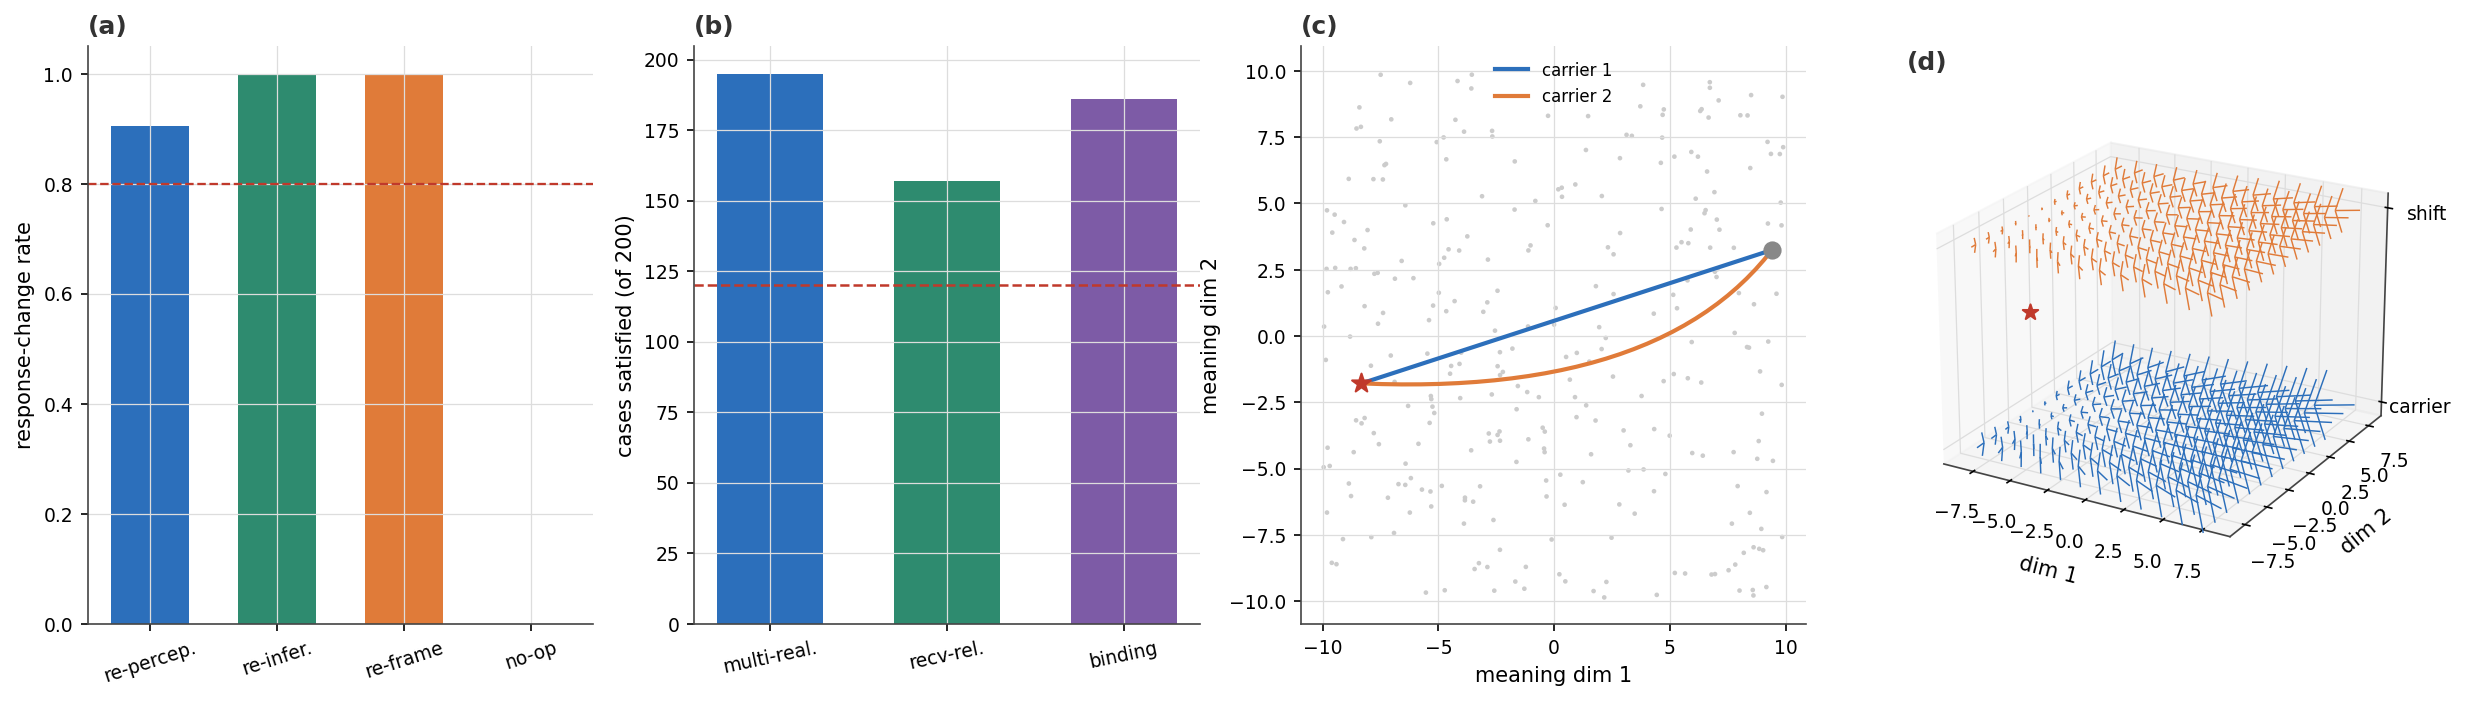
\includegraphics[width=\textwidth]{panels/panel_3.png}
    \caption{\textbf{The Advert Unit: Decoder Mechanisms and Carrier--Shift Decoupling.}
    (\textbf{A})~Response-change rate (fraction of 200 trials in which the mechanism
    successfully moved the receiver's response) on the linear $y$-axis for the four
    conditions on the $x$-axis: re-perception, re-inference, re-framing, and no-op.
    All three active mechanisms exceed the $80\%$ threshold (red dashed); the no-op
    leaves the response exactly unchanged in all 200 trials. Confirms
    Theorem~\ref{thm:decoderlocus} (Decoder Locus): the three mechanisms are
    exhaustive and mutually operative, and holding all three fixed leaves the
    response invariant.
    (\textbf{B})~Cases cleared (out of 200) on the linear $y$-axis for the three
    decoupling clauses on the $x$-axis: multiple realisability (multi-real.),
    receiver relativity (recv-rel.), and binding. All three exceed the threshold of
    120 cases (red dashed), confirming Theorem~\ref{thm:decoupling}
    (Carrier--Shift Decoupling): distinct carriers can induce the same shift; the
    same carrier induces different shifts across receivers; and carrier and shift are
    conjugate representations under the decoder.
    (\textbf{C})~Two carrier trajectories in meaning-space (two-dimensional, axes
    are decoder-output dimensions): carrier~1 (blue) and carrier~2 (orange) depart
    from the same source percept (star marker) and arrive at the same target
    cell (circle marker) via physically distinct paths through meaning-space.
    The paths differ; the endpoint cell is the same. Confirms the multiple
    realisability clause: different physical carriers realise the same decoder-shift
    into the target region.
    (\textbf{D})~Three-dimensional dual-representation view: the carrier acts in
    percept space (blue quiver field, lower plane) while the induced shift acts in
    meaning-space (orange quiver field, upper plane), connected by the decoder
    (vertical correspondence). The two fields are conjugate representations of a
    single categorical object, the content of Theorem~\ref{thm:decoupling}(iii)
    (Binding): $\Delta = \mathcal{D} \circ \mathsf{c} \circ \mathcal{D}^{-1}$ on
    the decoder's image.}
    \label{fig:panel3-advertunit}
\end{figure*}


\begin{figure*}[!htbp]
    \centering
    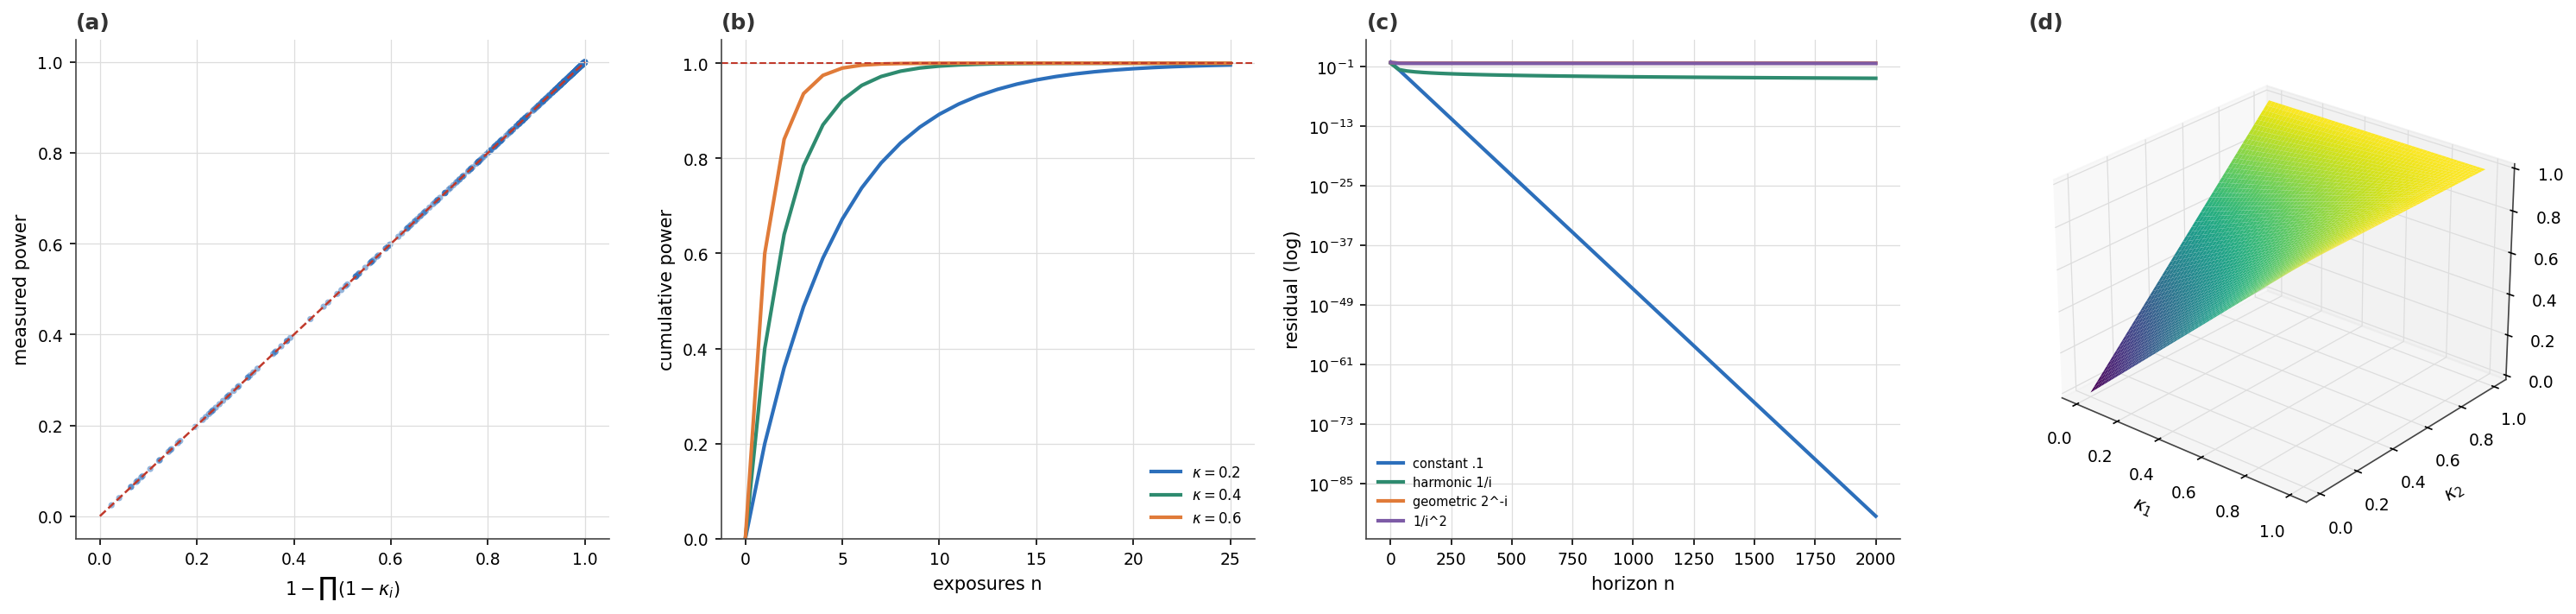
\includegraphics[width=\textwidth]{panels/panel_4.png}
    \caption{\textbf{The Calculus of Persuasive Power.}
    (\textbf{A})~Measured composite power (linear $y$-axis) versus the closed-form
    prediction $1 - \prod_{i}(1 - \kappa_i)$ (linear $x$-axis) across 500 random
    effect stacks. All points lie on the identity diagonal (red dashed) to
    floating-point precision (maximum deviation $2.2 \times 10^{-16}$), confirming
    Theorem~\ref{thm:multiplicative} (Multiplicative Law): the composite power of a
    stack of effects is exactly $1 - \prod_i(1 - \kappa_i)$.
    (\textbf{B})~Cumulative power $1 - (1 - \kappa)^n$ on the linear $y$-axis
    versus number of exposures $n$ (linear $x$-axis, 0 to 25) for three values of
    $\kappa$ (0.2, 0.4, 0.6). All three curves rise monotonically toward but never
    reach the ceiling at $1$ (red dashed). Marginal gains are strictly decreasing
    at every step, confirming Corollary~\ref{cor:diminishing} (Diminishing Returns)
    and Corollary~\ref{cor:frequency} (Frequency Saturation): repetition of a
    single effect yields bounded, geometrically decaying returns.
    (\textbf{C})~Residual above-floor distance (log-scale $y$-axis) versus campaign
    horizon $n$ (linear $x$-axis, 0 to 2000) for four power sequences: constant
    $\kappa = 0.1$ (divergent sum), harmonic $1/i$ (divergent sum), geometric
    $2^{-i}$ (convergent sum), and $p$-series $1/i^2$ (convergent sum). Divergent-sum
    sequences drive the residual steadily toward zero (still vanishing at the horizon);
    convergent-sum sequences plateau at a positive constant. Confirms
    Theorem~\ref{thm:saturation} (Campaign Saturation): a campaign saturates the
    cell if and only if $\sum_i \kappa_i = \infty$ (Borel--Cantelli dichotomy).
    (\textbf{D})~Three-dimensional composite-power surface
    $1 - (1 - \kappa_1)(1 - \kappa_2)$ over the $(\kappa_1, \kappa_2)$ plane, both
    axes on $[0, 1]$. The surface rises from zero at the origin to a saturating
    sheet that approaches but never touches the ceiling at $1$. The curvature
    reflects the multiplicative residual law: each additional effect closes a
    decreasing fraction of remaining distance.}
    \label{fig:panel4-power}
\end{figure*}


\begin{figure*}[!htbp]
    \centering
    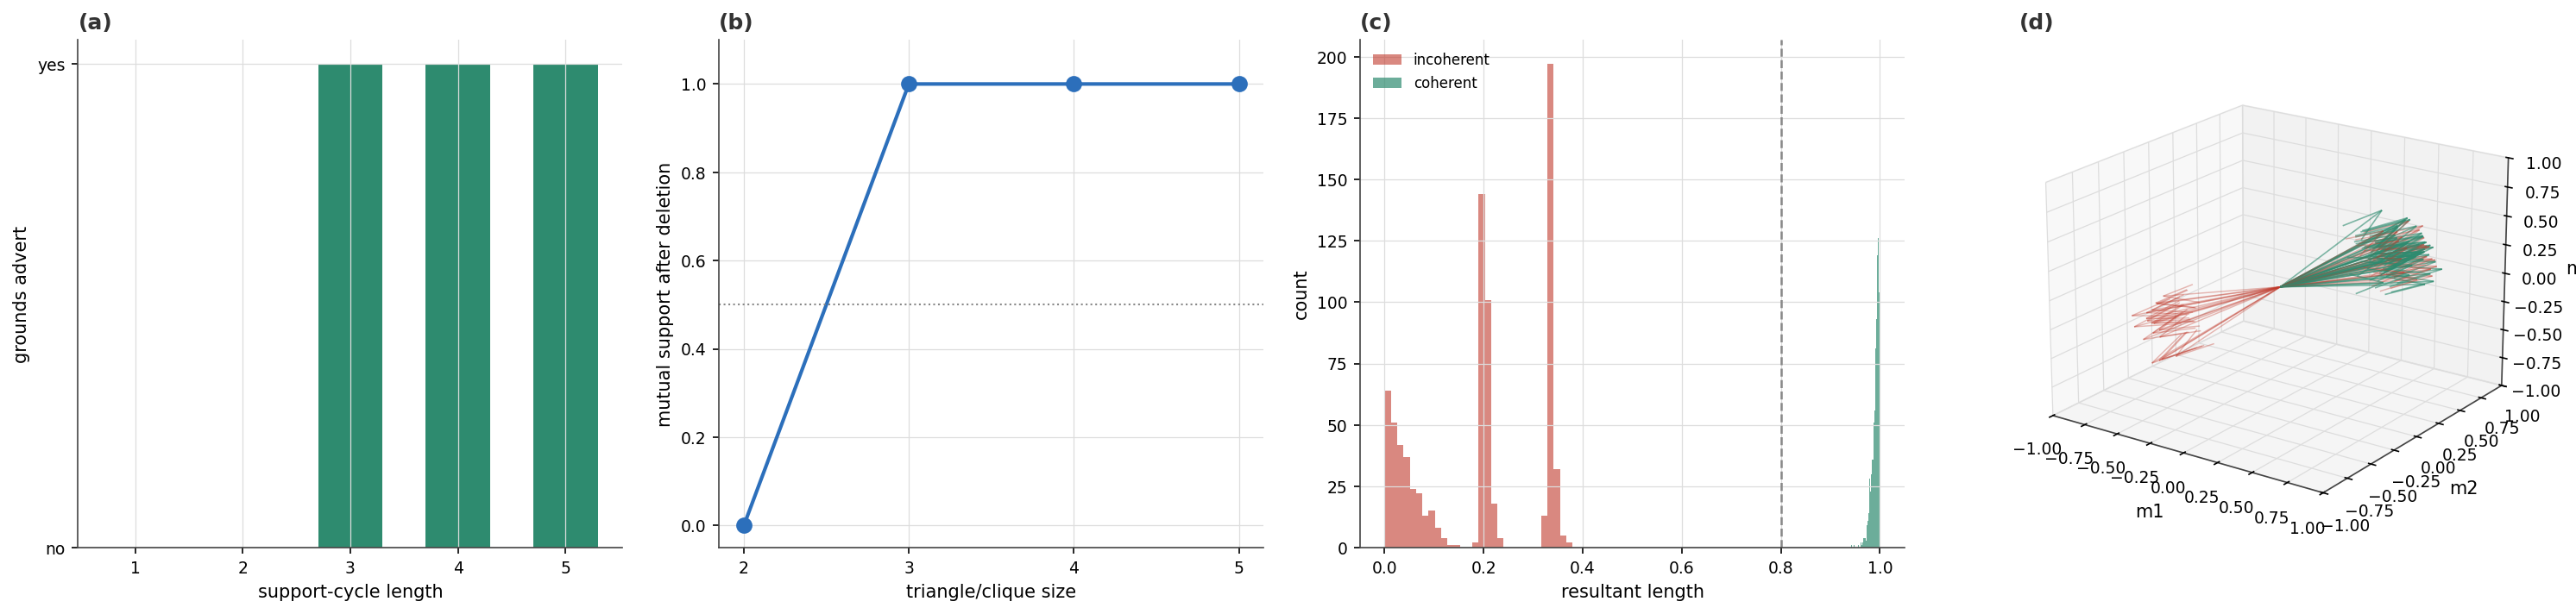
\includegraphics[width=\textwidth]{panels/panel_5.png}
    \caption{\textbf{Coherence: Grounding, Robustness, and Ordinal Detectability.}
    (\textbf{A})~Grounding outcome (yes/no, binary $y$-axis) versus support-cycle
    length (linear $x$-axis, 1 to 5) across 800 random support graphs. Cycles of
    length 1 and 2 fail to ground (all cases: no); cycles of length $\geq 3$ ground
    in every case (all cases: yes). Confirms Theorem~\ref{thm:triangle}(i)
    (Necessity): a grounded advert requires a directed cycle of length at least
    three in its support graph; self-support (length 1) and mutual-definition
    (length 2) are insufficient.
    (\textbf{B})~Mutual support surviving after deletion (linear $y$-axis, $[0,1]$)
    versus triangle or clique size (linear $x$-axis, 2 to 5). The 2-clique (mutual
    pair) drops to zero support on deletion of either element; the triangle (size 3)
    and larger cliques retain substantial mutual support above zero after any single
    deletion. Confirms Theorem~\ref{thm:triangle}(ii) (Sufficiency and Robustness):
    a strongly connected triangle at threshold $\theta > \frac{1}{2}$ is robust to
    single-effect removal.
    (\textbf{C})~Histogram of resultant shift length (linear $x$-axis) for
    incoherent adverts (red, left peak) and coherent adverts (green, right peak)
    across 2000 random adverts. The two distributions are well-separated: incoherent
    adverts have small resultant (effects pulling toward contradictory cells cancel)
    while coherent adverts have large resultant (effects reinforce toward one cell).
    A sign-only critic --- using only the sign of pairwise support, no magnitudes ---
    reproduced the magnitude-based verdict with 100\% agreement and flagged every
    incoherent advert. Confirms Corollary~\ref{cor:detect} (Ordinal Detectability):
    coherence is decidable from ordinal data alone.
    (\textbf{D})~Three-dimensional shift vector field in meaning-space $(m_1, m_2)$:
    coherent advert effects (green arrows) cluster and point toward a common
    terminus; incoherent advert effects (red/orange arrows) diverge toward
    contradictory directions. The separation is visible without any magnitude
    information, the spatial realisation of ordinal detectability.}
    \label{fig:panel5-coherence}
\end{figure*}
